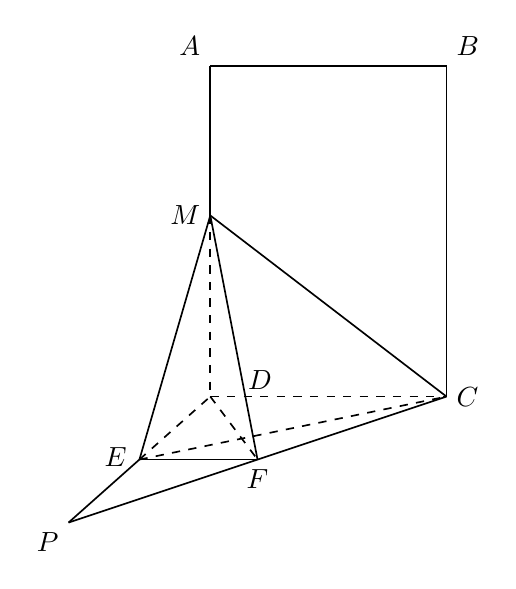
\begin{tikzpicture}[x=1cm,y=1cm,line width=0.6pt,font=\normalsize]
% rectangle ABCD frontal: A top-left, B top-right, C front-right, D back-left(base)
\coordinate (A) at (0,5.2);
\coordinate (B) at (3.0,5.2);
\coordinate (C) at (3.0,1.0);
\coordinate (D) at (0,1.0);
\coordinate (M) at (0.0000000000,3.3000000000);
\coordinate (E) at (-0.9000000000,0.2000000000);
\coordinate (F) at (0.6000000000,0.2000000000);
\coordinate (P) at (-1.8,-0.6);
% solid outer
\draw[solid] (A)--(B);
\draw[solid] (B)--(C);
\draw[solid] (A)--(M);
% folded solid tent
\draw[solid] (M)--(E);
\draw[solid] (M)--(F);
\draw[solid] (M)--(C);
\draw[solid] (E)--(F);
% original P triangle (fold source)
\draw[solid] (P)--(E);
\draw[solid] (P)--(F);
% hidden: M-D segment of AD, E-D segment of PD, F-C segment of PC, D-C, D-F
\draw[dashed] (M)--(D);
\draw[dashed] (E)--(D);
\draw[solid] (F)--(C);
\draw[dashed] (D)--(C);
\draw[dashed] (D)--(F);
% labels
\node[above left] at (A) {$A$};
\node[above right] at (B) {$B$};
\node[right] at (C) {$C$};
\node[right,xshift=10pt,yshift=6pt] at (D) {$D$};
\node[left] at (M) {$M$};
\node[left,xshift=-1.0pt,yshift=1.0pt] at (E) {$E$};
\node[below] at (F) {$F$};
\node[below left] at (P) {$P$};
\draw[dashed] (E)--(C);
\end{tikzpicture}
